\chapter{Avaliação}

Este capítulo fornece aplicações exemplos baseadas no ETL4NoSQL em dois domínios de naturezas distintas, utilizando SGBDs NoSQL para os dados de entrada. O desenvolvimento dessas aplicações pretende ilustrar a reusabilidade e flexibilidade do ETL4NoSQL em aplicações de ETL, que apresentam requisitos distintos de inserção e transformação de dados, e assim, avaliar o trabalho proposto neste documento.

Nas seções seguintes, são apresentadas as aplicações utilizadas como exemplo para a avaliação do nosso trabalho. Demonstraremos a implementação de duas aplicações de ETL estendidas do ETL4NoSQL, aplicando processos para extração, transformação e carga de dados modelando-os no esquema estrela, utilizando os dados de entrada armazenados no SBGD MongoDB e SGBD Cassandra.

\clearpage	

\section{Aplicações Baseadas no ETL4NoSQL}

Para avaliar o trabalho descrito neste documento, implementamos duas aplicações a partir do ETL4NoSQL. Elas são baseadas em dados sintéticos que podem ser encontrados em \cite{dataMongo} e \cite{dataCassandra}. 

Nossa motivação para escolha das duas aplicações foi para demonstrar a flexibilidade da ferramenta proposta ao lidar com SGBDs NoSQL de diferentes paradigmas, além dos SGBDs escolhidos serem bastante utilizados atualmente. Outra motivação foi facilitar a modelagem e carga desses dados no esquema estrela em DW.

Para a implementação, instanciamos a interface de leitura de dados (IDataMgr) e criamos as operações através da interface de operação (IOpMgr) de forma a modelar os dados, usando a interface de modelagem (IModelMgr), no esquema estrela. Finalmente, pudemos processar os dados por meio da interface de processamento (IProcMgr) e carregá-los em um arquivo de saída com o formato JSON.

Dessa forma, o uso das interfaces do \textit{framework} ETL4NoSQL auxilia o projetista de ETL na modelagem dos processos a partir de seu reuso, além de permitir adequar os processos de acordo com o seu domínio por meio da flexibilização das interfaces dos componentes do ETL4NoSQL.

Na seção seguinte, exibiremos o desenvolvimento da aplicação ETL4NoSQLMongoStar, que consiste em uma aplicação de ETL baseada no ETL4NoSQL utilizando o SGBD MongoDB como fonte de dados e o esquema estrela como modelo de dados para saída dos dados.

\section{Aplicação ETL4NoSQLMongoStar}

Para o desenvolvimento deste exemplo de aplicação utilizamos o SGBD MongoDB e uma base de dados que armazena a avaliação dos clientes de vários tipos de restaurantes. A seguir apresentamos a estrutura da base de dados utilizada nesta aplicação.

\begin{lstlisting}[frame=single, language=Oberon-2, basicstyle=\tiny]

{
	"address": {
		"building": "1007",
		"coord": [ -73.856077, 40.848447 ],
		"street": "Morris Park Ave",
		"zipcode": "10462"
	},
	"borough": "Bronx",
	"cuisine": "Bakery",
	"grades": [
		{ "date": { "$date": 1393804800000 }, "grade": "A", "score": 2 },
		{ "date": { "$date": 1378857600000 }, "grade": "A", "score": 6 },
		{ "date": { "$date": 1358985600000 }, "grade": "A", "score": 10 },
		{ "date": { "$date": 1322006400000 }, "grade": "A", "score": 9 },
		{ "date": { "$date": 1299715200000 }, "grade": "B", "score": 14 }
	],
	"name": "Morris Park Bake Shop",
	"restaurant_id": "30075445"
}

\end{lstlisting}  

Assim sendo, na figura \ref{mongomultidim} definimos o modelo multidimensional no esquema estrela para a esta estrutura de dados.

\begin{figure}[h!]
	\centering
	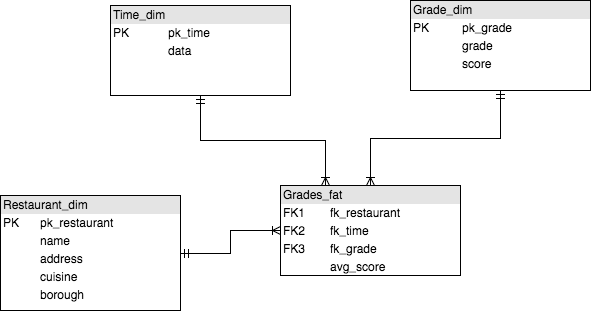
\includegraphics[scale=0.5]{fig/mongo_multidim.png}
	\caption{Modelo Multidimensional da aplicação ETL4NoSQLMongoStar}
	\label{mongomultidim}
\end{figure}

A partir do \textit{framework} ETL4NoSQL, pudemos estender uma nova aplicação denominada ETL4NoSQLMongoStar para desenvolver e executar os processos de ETL de forma a atender ao modelo multidimensional especificado para o exemplo utilizado.

\begin{figure}[h!]
	\centering
	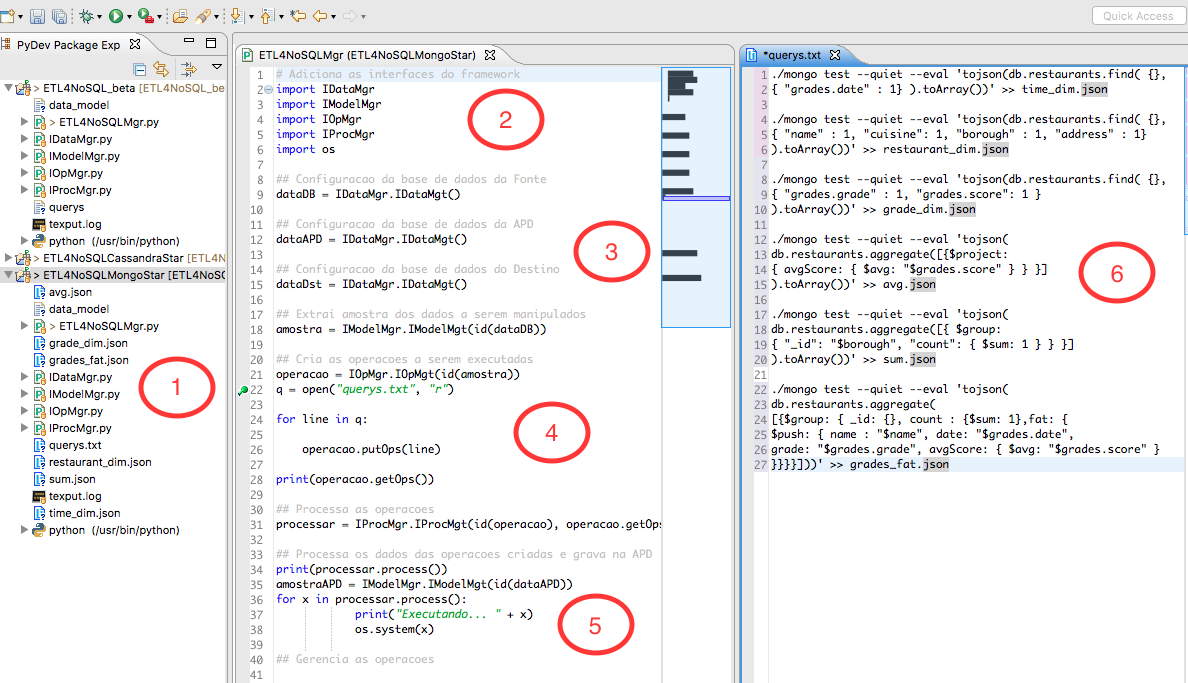
\includegraphics[scale=0.4]{fig/ETL4NoSQLMongoStar.png}
	\caption{Tela da aplicação ETL4NoSQLMongoStar}
	\label{etl4nosqlmongostar}
\end{figure}

Na figura \ref{etl4nosqlmongostar} podemos ver a aplicação ETL4NoSQLMongoStar, no destaque 1 temos a árvore de arquivos da aplicação, incluindo os arquivos de saída, criados ao final da execução dos processos de ETL. Já no destaque 2 é importada as interfaces dos componentes do \textit{framework}. No destaque 3 é feita a leitura das bases de dados envolvidas nos processos, no destaque 4 é realizada a inserção das operações a serem efetuadas e no destaque 5 os processos são executados. O destaque 6 apresenta as operações a serem efetivadas pelo \textit{framework} para criar o modelo multidimensional do ETL4NoSQLMongoStar e sua saída de dados em arquivos JSON.

A próxima seção disserta a respeito de outra aplicação de ETL estendida a partir do ETL4NoSQL, denominada ETL4NoSQLCassandraStar. Ela utiliza como fonte de dados o SGBD Cassandra e o esquema de dados estrela é o escolhido como modelo de dados para saída dos dados.


\section{Aplicação ETL4NoSQLCassandraStar}

A aplicação exemplo ETL4NoSQLCassandraStar foi criada a partir do \textit{framework} ETL4NoSQL proposto neste trabalho, utilizamos o SGBD Cassandra e a base de dados de localizações de táxis, de acordo com sua latitude e longitude em um determinado momento. A estrutura de dados da base de dados origem pode ser vista no código a seguir.

\begin{lstlisting}[frame=single, language=Oberon-2, basicstyle=\tiny]

	CREATE TABLE taxi.localizacoes (  
		taxi_id int, 
		date_time text,
		longitude text,
		latitude text 
	PRIMARY KEY (taxi_id));

\end{lstlisting}

Com isso, determinamos o modelo multidimensional seguindo o esquema estrela para esta estrutura de dados mostrada na figura \ref{cassandramultidim}.

\begin{figure}[h!]
	\centering
	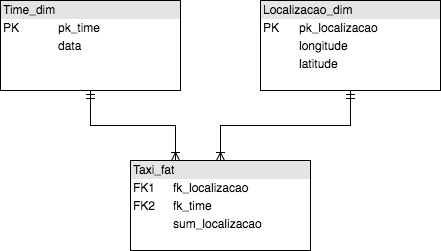
\includegraphics[scale=0.5]{fig/cassandra_multidim.png}
	\caption{Modelo Multidimensional da aplicação ETL4NoSQLCassandraStar}
	\label{cassandramultidim}
\end{figure}

Assim, utilizando a aplicação estendida do ETL4NoSQL, pudemos executar os processos de ETL para atender ao modelo multidimensional.

\begin{figure}[h!]
	\centering
	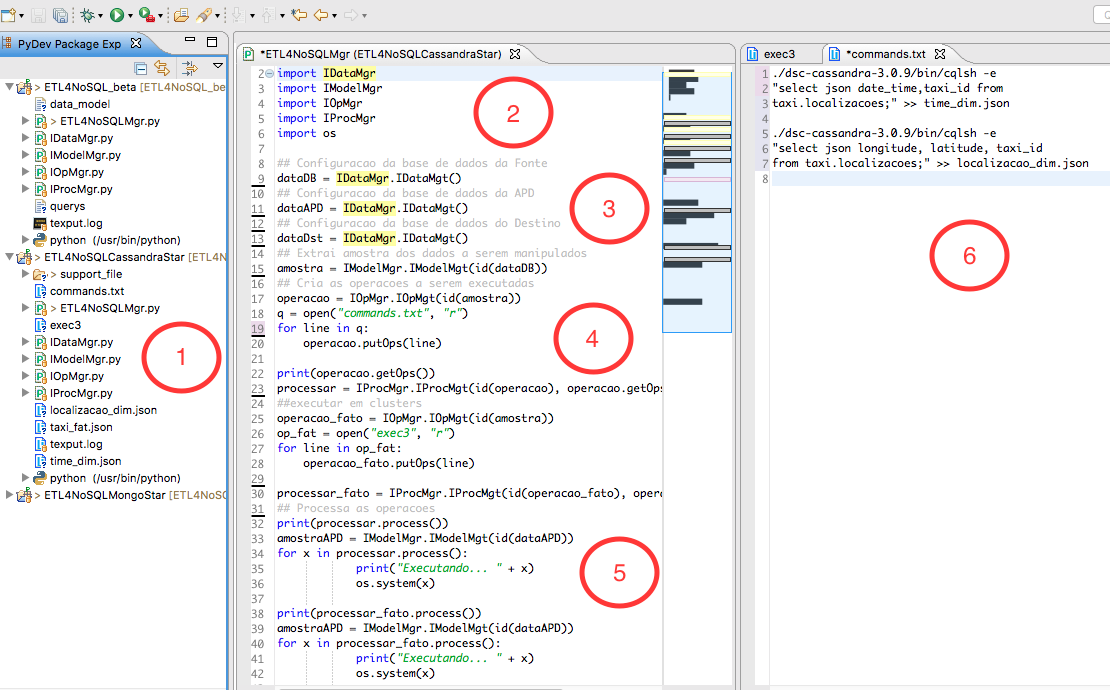
\includegraphics[scale=0.4]{fig/ETL4NoSQLCassandraStar.png}
	\caption{Tela da aplicação ETL4NoSQLCassandraStar}
	\label{ETL4NoSQLCassandraStar}
\end{figure}

Na figura \ref{ETL4NoSQLCassandraStar} podemos ver a aplicação ETL4NoSQLCassandraStar. Da mesma forma que a aplicação ETL4NoSQLMongoStar, no destaque 1 temos a árvore de arquivos da aplicação, incluindo os arquivos de saída, gerados ao final da execução dos processos de ETL. Já no destaque 2 é importada as interfaces dos componentes do \textit{framework}. No destaque 3 é feita a leitura das bases de dados envolvidas nos processos, no destaque 4 é realizada a inserção das operações a serem executadas e no destaque 5 os processos são efetivados. O destaque 6 apresenta as operações a serem efetuadas pelo \textit{framework} para criar o modelo multidimensional do ETL4NoSQLCassandraStar e sua saída de dados em arquivos JSON.

Por conseguinte, é importante ressaltar que para transformar os dados no esquema estrela utilizando aplicações estendidas do ETL4NoSQL, bastou apenas adicionar os parâmetros de consulta de cada SGBD NoSQL para executar os processos de busca, junção e escrita, demonstrando que o \textit{framework} proposto é programável, no sentido de possibilitar a programação dos seus parâmetros. Ele é reusável, pois permite que seus componentes sejam reutilizados por várias aplicações. E finalmente, flexível, dado que é possível estendê-lo para atender vários domínios de aplicação. 

  
\section{Considerações Finais}

Este capítulo evidenciou duas aplicações de naturezas distintas estendidas do ETL4NoSQL, avaliando suas características de reusabilidade e flexibilidade. Uma aplicação foi baseada no SGBD NoSQL Mongo e a outra no SGBD NoSQL Cassandra. Utilizamos o ETL4NoSQLCassandraStar e o ETL4NoSQLMongoStar para desenvolver e executar os processos. Ao final da execução dos processos pudemos gerar um arquivo de saída em formato comum, denominado JSON. 

No capítulo posterior, esta pesquisa é finalizada, expondo as principais contribuições, discussões sobre dificuldades e as ameaças do trabalho de pesquisa, os resultados e trabalhos futuros a partir do ETL4NoSQL.
